\chapter{Backtracking}

\section{Regular Expression Matching} %%%%%%%%%%%%%%%%%%%%%%

\subsubsection{Description}
Implement regular expression matching with support for \fn{'.'} and \fn{'*'}.

\fn{'.'} Matches any single character.
\fn{'*'} Matches zero or more of the preceding element.

The matching should cover the entire input string (not partial).

Some examples:
\begin{Code}
isMatch("aa","a") → false
isMatch("aa","aa") → true
isMatch("aaa","aa") → false
isMatch("aa", "a*") → true
isMatch("aa", ".*") → true
isMatch("ab", ".*") → true
isMatch("aab", "c*a*b") → true
\end{Code}

\subsubsection{Solution}

\begin{Code}
public boolean isMatch(String s, String p) {
    if (p.isEmpty()) {
        return s.isEmpty();
    } else if (p.length() == 1) {
        return s.length() == 1 && isEqual(s, p);
    } else if (p.charAt(1) != '*') {
        return s.length() > 0 && isEqual(s, p) && isMatch(s.substring(1), p.substring(1));
    } else {
        if (s.length() > 0 && isEqual(s, p)) {
            return isMatch(s, p.substring(2)) || isMatch(s.substring(1), p);
        } else {
            return isMatch(s, p.substring(2));
        }
    }
}

private boolean isEqual(String s, String p) {
    return s.charAt(0) == p.charAt(0) || p.charAt(0) == '.';
}
\end{Code}

\newpage

\section{Wildcard Matching} %%%%%%%%%%%%%%%%%%%%%%

\subsubsection{Description}
Implement wildcard pattern matching with support for \fn{'?'} and \fn{'*'}.

\fn{'?'} Matches any single character.
\fn{'*'} Matches any sequence of characters (including the empty sequence).

\begin{Code}
Some examples:
isMatch("aa","a") → false
isMatch("aa","aa") → true
isMatch("aaa","aa") → false
isMatch("aa", "*") → true
isMatch("aa", "a*") → true
isMatch("ab", "?*") → true
isMatch("aab", "c*a*b") → false
\end{Code}

\subsubsection{Solution}
\begin{Code}
public boolean isMatch2(String s, String p) {
    int is = 0, ip = 0, ks = -1, kp = -1;

    while (is < s.length()) {
        if (ip < p.length() && (s.charAt(is) == p.charAt(ip) || p.charAt(ip) == '?')) {
            is++;
            ip++;
        } else if (ip < p.length() && p.charAt(ip) == '*') {
            ks = is;
            kp = ip;
            ip++;
        } else if (kp != -1) {
            is = ++ks;
            ip = kp + 1;
        } else {
            return false;
        }
    }

    for ( ; ip < p.length() && p.charAt(ip) == '*'; ip++);
    return ip == p.length();
}
\end{Code}

\newpage

\section{Letter solution.Combinations of a Phone Number} %%%%%%%%%%%%%%%%%%%%%%

\subsubsection{Description}
Given a digit string, return all possible letter combinations that the number could represent.

A mapping of digit to letters (just like on the telephone buttons) is given below.

\begin{center}
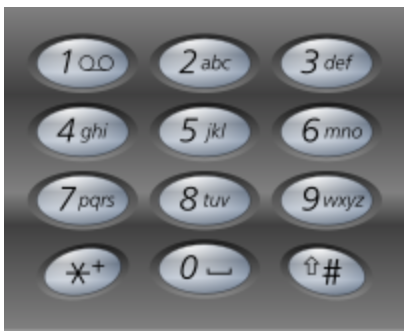
\includegraphics[width=150pt]{phone.png}\\
\figcaption{Phone Keyboard}\label{fig:phone-keyboard}
\end{center}

\textbf{Input:} Digit string \code{"23"}

\textbf{Output:} \code{["ad", "ae", "af", "bd", "be", "bf", "cd", "ce", "cf"]}.

\subsubsection{Solution I}

\begin{Code}
private final String[] ARR = {
        "", "", "abc", "def", "ghi", "jkl", "mno", "pqrs", "tuv", "wxyz"
};

public List<String> letterCombinations(String digits) {
    List<String> list = new LinkedList<>();
    if (!digits.isEmpty()) {
        helper(digits, 0, list, "");
    }
    return list;
}

private void helper(String digits, int start, List<String> list, String s) {
    if (start >= digits.length()) {
        list.add(s);
        return;
    }
    int n = digits.charAt(start) - '0';
    for (char c : ARR[n].toCharArray()) {
        helper(digits, start + 1, list, s + c);
    }
}
\end{Code}

\newpage

\subsubsection{Solution II}

\begin{Code}

public List<String> letterCombinations(String digits) {
    LinkedList<String> queue = new LinkedList<String>();
    if (digits.length() == 0) {
        return queue;
    }

    Queue<String> next = new LinkedList<>();
    queue.add("");

    for (int i = 0; i < digits.length() && !queue.isEmpty(); ) {
        String s = queue.poll();
        int n = digits.charAt(i) - '0';
        for (char c : ARR[n].toCharArray()) {
            next.add(s + c);
        }
        if (queue.isEmpty()) {
            queue.addAll(next);
            next.clear();
            i++;
        }
    }
    return queue;
}
\end{Code}

\newpage

\section{Generate Parentheses} %%%%%%%%%%%%%%%%%%%%%%

\subsubsection{Description}
Given n pairs of parentheses, write a function to generate all combinations of well-formed parentheses.

For example, given \code{n = 3}, a solution set is:
\begin{Code}
[
  "((()))",
  "(()())",
  "(())()",
  "()(())",
  "()()()"
]
\end{Code}

\subsubsection{Solution}

\begin{Code}
public List<String> generateParenthesis(int n) {
    List<String> result = new LinkedList<String>();
    dfs(result, n, "", 0, 0);
    return result;
}

private void dfs(List<String> result, int n, String str, int left, int right) {
    if (left == n && right == n) {
        result.add(str);
        return;
    }
    if (left > n || right > n || left < right) {
        return;
    }
    dfs(result, n, str + "(", left + 1, right);
    dfs(result, n, str + ")", left, right + 1);
}
\end{Code}

\newpage

\section{solution.Permutations} %%%%%%%%%%%%%%%%%%%%%%

\subsubsection{Description}
Given a collection of distinct numbers, return all possible permutations.

For example, \code{[1,2,3]} have the following permutations:
\begin{Code}
[
  [1,2,3],
  [1,3,2],
  [2,1,3],
  [2,3,1],
  [3,1,2],
  [3,2,1]
]
\end{Code}

\subsubsection{Solution}
\begin{Code}
public List<List<Integer>> permute(int[] nums) {
    List<List<Integer>> result = new ArrayList<List<Integer>>();
    permute(nums, result, 0);
    return result;
}

public void permute(int[] nums, List<List<Integer>> result, int start) {
    if (start >= nums.length) {
        List<Integer> list = new ArrayList<Integer>();
        for (Integer n : nums) {
            list.add(n);
        }
        result.add(list);
    }

    for (int i = start; i < nums.length; i++) {
        swap(nums, start, i);
        permute(nums, result, start + 1);
        swap(nums, start, i);
    }
}

public static void swap(int[] nums, int left, int right) {
    int temp = nums[left];
    nums[left] = nums[right];
    nums[right] = temp;
}
\end{Code}

\newpage

\section{solution.Permutations II} %%%%%%%%%%%%%%%%%%%%%%

\subsubsection{Description}

Given a collection of numbers that might contain duplicates, return all possible unique permutations.

For example,

\code{[1,1,2]} have the following unique permutations:
\begin{Code}
[
  [1,1,2],
  [1,2,1],
  [2,1,1]
]
\end{Code}

\subsubsection{Solution}

\begin{Code}
public List<List<Integer>> permuteUnique(int[] nums) {
    List<List<Integer>> result = new ArrayList<List<Integer>>();
    permute(nums, result, 0);
    return result;
}

public void permute(int[] nums, List<List<Integer>> result, int start) {
    if (start >= nums.length) {
        List<Integer> list = new ArrayList<Integer>();
        for (Integer n : nums) {
            list.add(n);
        }
        result.add(list);
    }

    HashSet<Integer> set = new HashSet<Integer>();
    for (int i = start; i < nums.length; i++) {
        if (set.add(nums[i])) {
            swap(nums, start, i);
            permute(nums, result, start + 1);
            swap(nums, start, i);
        }
    }
}

public static void swap(int[] nums, int left, int right) {
    int temp = nums[left];
    nums[left] = nums[right];
    nums[right] = temp;
}
\end{Code}

\newpage

\section{Permutation Sequence} %%%%%%%%%%%%%%%%%%%%%%

\subsubsection{Description}
The set \code{[1,2,3,…,n]} contains a total of \code{n!} unique permutations.

By listing and labeling all of the permutations in order,
We get the following sequence (ie, for n = 3):
\begin{Code}
"123"
"132"
"213"
"231"
"312"
"321"
\end{Code}

Given n and k, return the kth permutation sequence.

Note: Given n will be between 1 and 9 inclusive.

\subsubsection{Solution}

\begin{Code}
public String getPermutation(int n, int k) {
    int[] fac = new int[n + 1];
    fac[0] = 1;

    List<Integer> list = new LinkedList<>();

    for (int i = 1; i <= n; i++) {
        fac[i] = fac[i - 1] * i;
        list.add(i);
    }

    k--;

    StringBuilder sb = new StringBuilder();
    for (int i = 1; i <= n; i++) {
        int ind = k / fac[n - i];
        k %= fac[n - i];
        sb.append(list.remove(ind));
    }

    return sb.toString();
}
\end{Code}

\newpage


\section{Word Search} %%%%%%%%%%%%%%%%%%%%%%

\subsubsection{Description}
Given a 2D board and a word, find if the word exists in the grid.

The word can be constructed from letters of sequentially adjacent cell, where adjacent cells are those horizontally or vertically neighboring. The same letter cell may not be used more than once.

For example,
Given board =
\begin{Code}
[
  ['A','B','C','E'],
  ['S','F','C','S'],
  ['A','D','E','E']
]
\end{Code}

word = \code{"ABCCED"}, -> returns true,

word = \code{"SEE"}, -> returns true,

word = \code{"ABCB"}, -> returns false.

\subsubsection{Solution}

\begin{Code}
public boolean exist(char[][] board, String word) {
    for (int i = 0; i < board.length; i++) {
        for (int j = 0; j < board[0].length; j++) {
            if (dfs(board, i, j, word, 0)) {
                return true;
            }
        }
    }
    return false;
}

private boolean dfs(char[][] board, int i, int j, String word, int start) {
    if (start == word.length()) {
        return true;
    }
    if (i < 0 || i >= board.length || j < 0 || j >= board[0].length) {
        return false;
    }
    if (board[i][j] != word.charAt(start)) {
        return false;
    }

    board[i][j] ^= '#';
    boolean flag = dfs(board, i + 1, j, word, start + 1)
            || dfs(board, i - 1, j, word, start + 1)
            || dfs(board, i, j + 1, word, start + 1)
            || dfs(board, i, j - 1, word, start + 1);
    board[i][j] ^= '#';
    return flag;
}
\end{Code}

\newpage

\section{Word Search II} %%%%%%%%%%%%%%%%%%%%%%

\subsubsection{Description}
Given a 2D board and a list of words from the dictionary, find all words in the board.

Each word must be constructed from letters of sequentially adjacent cell, where adjacent cells are those horizontally or vertically neighboring. The same letter cell may not be used more than once in a word.

For example,
Given words = \code{["oath","pea","eat","rain"]} and board =
\begin{Code}
[
  ['o','a','a','n'],
  ['e','t','a','e'],
  ['i','h','k','r'],
  ['i','f','l','v']
]
\end{Code}
Return \code{["eat","oath"]}.

Note:
You may assume that all inputs are consist of lowercase letters a-z.

You would need to optimize your backtracking to pass the larger test. Could you stop backtracking earlier?

If the current candidate does not exist in all words' prefix, you could stop backtracking immediately. What kind of data structure could answer such query efficiently? Does a hash table work? Why or why not? How about a solution.Trie? If you would like to learn how to implement a basic trie, please work on this problem: Implement solution.Trie (Prefix Tree) first.

\subsubsection{Solution}

\begin{Code}
private class solution.Trie {
    solution.Trie[] nodes = new solution.Trie[26];
    String word;
}

private void buildTrie(solution.Trie trie, String word) {
    for (int i = 0; i < word.length(); i++) {
        if (trie.nodes[word.charAt(i) - 'a'] == null) {
            trie.nodes[word.charAt(i) - 'a'] = new solution.Trie();
        }
        trie = trie.nodes[word.charAt(i) - 'a'];
    }
    trie.word = word;
}

\end{Code}

\newpage

\begin{Code}
public List<String> findWords(char[][] board, String[] words) {
    solution.Trie trie = new solution.Trie();
    for (String word : words) {
        buildTrie(trie, word);
    }
    Set<String> set = new HashSet<String>();
    for (int i = 0; i < board.length; i++) {
        for (int j = 0; j < board[0].length; j++) {
            dfs(set, board, i, j, trie);
        }
    }
    return new LinkedList<String>(set);
}

private void dfs(Set<String> set, char[][] board, int i, int j, solution.Trie trie) {
    if (i < 0 || i >= board.length || j < 0 || j >= board[0].length) {
        return;
    }
    if (trie == null) {
        return;
    }
    char c = board[i][j];
    if (c < 'a' || c > 'z') {
        return;
    }
    trie = trie.nodes[c - 'a'];
    if (trie == null) {
        return;
    }
    if (trie.word != null) {
        set.add(trie.word);
    }

    board[i][j] ^= '#';
    dfs(set, board, i + 1, j, trie);
    dfs(set, board, i - 1, j, trie);
    dfs(set, board, i, j + 1, trie);
    dfs(set, board, i, j - 1, trie);
    board[i][j] ^= '#';
}
\end{Code}

\newpage

\section{Word Break II} %%%%%%%%%%%%%%%%%%%%%%

\subsubsection{Description}
Given a non-empty string s and a dictionary wordDict containing a list of non-empty words, add spaces in s to construct a sentence where each word is a valid dictionary word. You may assume the dictionary does not contain duplicate words.

Return all such possible sentences.

For example, given
s = \code{"catsanddog"},
dict = \code{["cat", "cats", "and", "sand", "dog"]}.

A solution is \code{["cats and dog", "cat sand dog"]}.

\subsubsection{Solution}

\begin{Code}
public List<String> wordBreak(String s, List<String> wordDict) {
    HashMap<String, List<String>> cache = new HashMap<>();
    cache.put("", Arrays.asList(""));
    return dfs(s, new HashSet<String>(wordDict), cache);
}

List<String> dfs(String s, HashSet<String> wordDict, HashMap<String, List<String>> cache) {
    if (cache.containsKey(s)) {
        return cache.get(s);
    }
    List<String> result = new LinkedList<>();
    for (int i = 0; i < s.length(); i++) {
        String t = s.substring(i);
        if (wordDict.contains(t)) {
            List<String> list = dfs(s.substring(0, i), wordDict, cache);
            if (list != null) {
                for (String ss : list) {
                    result.add((ss.length() > 0 ? ss + " " : "") + t);
                }
            }
        }
    }
    cache.put(s, result);
    return result;
}
\end{Code}

\newpage

\section{Combination Sum} %%%%%%%%%%%%%%%%%%%%%%

\subsubsection{Description}

Given a set of candidate numbers (C) (without duplicates) and a target number (T), find all unique combinations in C where the candidate numbers sums to T.

The same repeated number may be chosen from C unlimited number of times.

Note:

All numbers (including target) will be positive integers.

The solution set must not contain duplicate combinations.

For example, given candidate set \code{[2, 3, 6, 7]} and target 7,

A solution set is:
\begin{code}
[
  [7],
  [2, 2, 3]
]
\end{code}

\subsubsection{Solution I}

\begin{Code}
public List<List<Integer>> combinationSum(int[] candidates, int target) {
    List<List<Integer>> result = new LinkedList<>();
    helper(candidates, result, new LinkedList<>(), target, 0);
    return result;
}

void helper(int[] candidates, List<List<Integer>> result, List<Integer> list, int target, int index) {
    if (target < 0) {
        return;
    } else if (target == 0) {
        result.add(new LinkedList<>(list));
        return;
    } else if (index >= candidates.length) {
        return;
    }

    list.add(candidates[index]);
    helper(candidates, result, list, target - candidates[index], index);
    list.remove(list.size() - 1);

    helper(candidates, result, list, target, index + 1);
}
\end{Code}

\newpage

\subsubsection{Solution II}

\begin{Code}

public List<List<Integer>> combinationSum(int[] candidates, int target) {
    List<List<Integer>> result = new LinkedList<>();
    dfs(candidates, target, 0, result, new LinkedList<Integer>());
    return result;
}

void dfs(int[] candidates, int target, int start, List<List<Integer>> result, List<Integer> list) {
    if (target < 0) {
        return;
    }
    if (target == 0) {
        result.add(new LinkedList<>(list));
        return;
    }
    for (int i = start; i < candidates.length; i++) {
        list.add(candidates[i]);
        dfs(candidates, target - candidates[i], i, result, list);
        list.remove(list.size() - 1);
    }
}
\end{Code}

\newpage

\section{Combination Sum II} %%%%%%%%%%%%%%%%%%%%%%

\subsubsection{Description}
Given a collection of candidate numbers (C) and a target number (T), find all unique combinations in C where the candidate numbers sums to T.

Each number in C may only be used once in the combination.

Note:

All numbers (including target) will be positive integers.

The solution set must not contain duplicate combinations.

For example, given candidate set \code{[10, 1, 2, 7, 6, 1, 5]} and target 8,

A solution set is:
\begin{Code}
[
  [1, 7],
  [1, 2, 5],
  [2, 6],
  [1, 1, 6]
]
\end{Code}

\subsubsection{Solution I}

\begin{Code}
public List<List<Integer>> combinationSum(int[] candidates, int target) {
    List<List<Integer>> result = new LinkedList<>();
    Arrays.sort(candidates);
    helper(candidates, result, new LinkedList<>(), target, 0);
    return result;
}

void helper(int[] candidates, List<List<Integer>> result, List<Integer> list, int target, int index) {
    if (target < 0) {
        return;
    } else if (target == 0) {
        result.add(new LinkedList<>(list));
        return;
    } else if (index >= candidates.length) {
        return;
    }

    list.add(candidates[index]);
    helper(candidates, result, list, target - candidates[index], index + 1);
    list.remove(list.size() - 1);

    for ( ; index < candidates.length - 1 && candidates[index + 1] == candidates[index]; index++);

    helper(candidates, result, list, target, index + 1);
}
\end{Code}

\newpage

\subsubsection{Solution II}

\begin{Code}
public List<List<Integer>> combinationSum(int[] candidates, int target) {
    List<List<Integer>> result = new LinkedList<List<Integer>>();
    Arrays.sort(candidates);
    dfs(candidates, 0, target, result, new LinkedList<Integer>());
    return result;
}

void dfs(int[] candidates, int start, int target, List<List<Integer>> result, List<Integer> path) {
    if (target < 0) {
        return;
    }

    if (target == 0) {
        result.add(new LinkedList<Integer>(path));
        return;
    }

    for (int i = start; i < candidates.length; i++) {
        if (i > start && candidates[i] == candidates[i - 1]) {
            continue;
        }

        path.add(candidates[i]);

        // 关键是这里变成i + 1
        dfs(candidates, i + 1, target - candidates[i], result, path);
        path.remove(path.size() - 1);
    }
}
\end{Code}

\newpage

\section{Combination Sum III} %%%%%%%%%%%%%%%%%%%%%%

\subsubsection{Description}
Find all possible combinations of k numbers that add up to a number n, given that only numbers from 1 to 9 can be used and each combination should be a unique set of numbers.

\textbf{Example 1:}

Input: \code{k = 3, n = 7}

Output: \code{[[1,2,4]]}

\textbf{Example 2:}

Input: \code{k = 3, n = 9}

Output: \code{[[1,2,6], [1,3,5], [2,3,4]]}

\subsubsection{Solution I}

\begin{Code}
public List<List<Integer>> combinationSum(int k, int n) {
    List<List<Integer>> result = new LinkedList<>();
    helper(k, n, result, new LinkedList<>(), 1);
    return result;
}

private void helper(int k, int n, List<List<Integer>> result, List<Integer> list, int cur) {
    if (n == 0 && k == 0) {
        result.add(new LinkedList<>(list));
        return;
    }

    if (cur > 9) {
        return;
    }

    list.add(cur);
    helper(k - 1, n - cur, result, list, cur + 1);
    list.remove(list.size() - 1);

    helper(k, n, result, list, cur + 1);
}
\end{Code}

\newpage

\subsubsection{Solution II}

\begin{Code}
public List<List<Integer>> combinationSum(int k, int n) {
    List<List<Integer>> result = new LinkedList<>();
    dfs(n, k, 1, result, new LinkedList<Integer>());
    return result;
}

private void dfs(int target, int k, int start, List<List<Integer>> result, List<Integer> list) {
    if (target == 0 && k == 0) {
        result.add(new LinkedList<>(list));
        return;
    }
    if (target <= 0 || k <= 0) {
        return;
    }
    for (int i = start; i <= 9; i++) {
        list.add(i);
        dfs(target - i, k - 1, i + 1, result, list);
        list.remove(list.size() - 1);
    }
}
\end{Code}

\newpage

\section{Combination Sum IV} %%%%%%%%%%%%%%%%%%%%%%

\subsubsection{Description}
Given an integer array with all positive numbers and no duplicates, find the number of possible combinations that add up to a positive integer target.

\textbf{Example:}

nums = \code{[1, 2, 3]}
target = 4

The possible combination ways are:
\begin{Code}
(1, 1, 1, 1)
(1, 1, 2)
(1, 2, 1)
(1, 3)
(2, 1, 1)
(2, 2)
(3, 1)
\end{Code}

Note that different sequences are counted as different combinations.

Therefore the output is 7.

\textbf{Follow up:}

What if negative numbers are allowed in the given array?

How does it change the problem?

What limitation we need to add to the question to allow negative numbers?

\subsubsection{Solution}

\begin{Code}
public int combinationSum4(int[] nums, int target) {
    int[] dp = new int[target + 1];
    // 这里排序便于之后break
    Arrays.sort(nums);
    // 这里0为什么是1呢,我开始也不解,
    // 其实就是说如果组合中带的刚好是当前数,那么组合数只有1种。
    // 比如target为3的时候,遍历到了nums中的3,那么只有1种可能。
    dp[0] = 1;
    for (int i = 1; i <= target; i++) {
        for (int num : nums) {
            if (num > i) {
                break;
            } else {
                dp[i] += dp[i - num];
            }
        }
    }
    return dp[target];
}
\end{Code}

\newpage

\section{N-Queens} %%%%%%%%%%%%%%%%%%%%%%

\subsubsection{Description}
The n-queens puzzle is the problem of placing n queens on an n×n chessboard such that no two queens attack each other.

\begin{center}
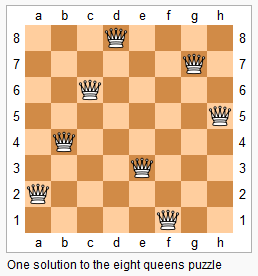
\includegraphics[width=150pt]{8-queens.png}\\
\end{center}

Given an integer n, return all distinct solutions to the n-queens puzzle.

Each solution contains a distinct board configuration of the n-queens' placement, where \code{'Q'} and \fn{'.'} both indicate a queen and an empty space respectively.

For example,

There exist two distinct solutions to the 4-queens puzzle:

\begin{Code}
[
 [".Q..",  // Solution 1
  "...Q",
  "Q...",
  "..Q."],

 ["..Q.",  // Solution 2
  "Q...",
  "...Q",
  ".Q.."]
]
\end{Code}

\newpage

\subsubsection{Solution}

\begin{Code}
public List<List<String>> solveNQueens(int n) {
    List<List<String>> result = new LinkedList<>();
    /**
     * 这里f[i]表示第i行皇后应该放置在第几列
     */
    int[] f = new int[n];
    dfs(f, result, 0);
    return result;
}

private void dfs(int[] f, List<List<String>> result, int row) {
    if (row == f.length) {
        List<String> list = new LinkedList<>();
        char[] c = new char[f.length];
        for (int i = 0; i < f.length; i++) {
            Arrays.fill(c, '.');
            for (int j = 0; j < f.length; j++) {
                if (j == f[i]) {
                    c[j] = 'Q';
                    break;
                }
            }
            list.add(String.valueOf(c));
        }
        result.add(list);
    }
    /**
     * 对于当前第row行,一列一列地尝试放置皇后,看是否合法,j表示列,如果合法则保存到f中
     */
    for (int j = 0; j < f.length; j++) {
        if (isValid(f, row, j)) {
            f[row] = j;
            dfs(f, result, row + 1);
        }
    }
}

private boolean isValid(int[] f, int row, int col) {
    for (int i = 0; i < row; i++) {
        if (f[i] == col) {
            return false;
        }
        if (Math.abs(i - row) == Math.abs(f[i] - col)) {
            return false;
        }
    }
    return true;
}
\end{Code}

\newpage

\section{N-Queens II} %%%%%%%%%%%%%%%%%%%%%%

\subsubsection{Description}

Follow up for N-Queens problem.

Now, instead outputting board configurations, return the total number of distinct solutions.

\subsubsection{Solution}

\begin{Code}
private int total;

public int totalNQueens(int n) {
    int[] f = new int[n];
    dfs(f, 0);
    return total;
}

private void dfs(int[] f, int row) {
    if (row == f.length) {
        total++;
        return;
    }
    for (int j = 0; j < f.length; j++) {
        if (isValid(f, row, j)) {
            f[row] = j;
            dfs(f, row + 1);
        }
    }
}

private boolean isValid(int[] f, int row, int col) {
    for (int i = 0; i < row; i++) {
        if (f[i] == col) {
            return false;
        }
        if (Math.abs(i - row) == Math.abs(f[i] - col)) {
            return false;
        }
    }
    return true;
}
\end{Code}

\newpage

\section{solution.Subsets} %%%%%%%%%%%%%%%%%%%%%%

\subsubsection{Description}

Given a set of distinct integers, nums, return all possible subsets.

Note: The solution set must not contain duplicate subsets.

For example,
If nums = \code{[1,2,3]}, a solution is:

\begin{Code}
[
  [3],
  [1],
  [2],
  [1,2,3],
  [1,3],
  [2,3],
  [1,2],
  []
]
\end{Code}

\subsubsection{Solution I}

\begin{Code}
public List<List<Integer>> subsets(int[] nums) {
    List<List<Integer>> result = new LinkedList<List<Integer>>();

    if (nums.length == 0) {
        return result;
    }

    subsets(nums, 0, result, new LinkedList<Integer>());

    return result;
}

private void subsets(int[] nums, int start, List<List<Integer>> list, List<Integer> path) {
    if (start == nums.length) {
        list.add(new LinkedList<Integer>(path));
        return;
    }

    path.add(nums[start]);
    subsets(nums, start + 1, list, path);
    path.remove(path.size() - 1);

    subsets(nums, start + 1, list, path);
}
\end{Code}

\newpage

\subsubsection{Solution II}

\begin{Code}
public List<List<Integer>> subsets(int[] nums) {
    List<List<Integer>> result = new LinkedList<List<Integer>>();

    if (nums.length == 0) {
        return result;
    }

    Arrays.sort(nums);
    subsets(nums, 0, result, new LinkedList<Integer>());
    return result;
}

private void subsets(int[] nums, int start, List<List<Integer>> result, List<Integer> path) {
    result.add(new LinkedList<Integer>(path));
    for (int i = start; i < nums.length; i++) {
        path.add(nums[i]);
        subsets(nums, i + 1, result, path);
        path.remove(path.size() - 1);
    }
}
\end{Code}

\newpage

\section{solution.Subsets II} %%%%%%%%%%%%%%%%%%%%%%

\subsubsection{Description}
Given a collection of integers that might contain duplicates, nums, return all possible subsets.

Note: The solution set must not contain duplicate subsets.

For example,
If nums = \code{[1,2,2]}, a solution is:

\begin{Code}
[
  [2],
  [1],
  [1,2,2],
  [2,2],
  [1,2],
  []
]
\end{Code}

\subsubsection{Solution}

\begin{Code}
public List<List<Integer>> subsetsWithDup(int[] nums) {
    List<List<Integer>> result = new LinkedList<List<Integer>>();

    if (nums.length == 0) {
        return result;
    }
    /**
     * 千万别掉了排序
     */
    Arrays.sort(nums);
    subsetsWithDup(nums, 0, result, new LinkedList<Integer>());

    return result;
}

private void subsetsWithDup(int[] nums, int start, List<List<Integer>> list, List<Integer> path) {
    if (start == nums.length) {
        list.add(new LinkedList<Integer>(path));
        return;
    }

    path.add(nums[start]);
    subsetsWithDup(nums, start + 1, list, path);
    path.remove(path.size() - 1);

    // 既然不带当前字符,那后面如果重复的都别带,否则就是带了当前字符的子集
    for ( ; start + 1 < nums.length && nums[start + 1] == nums[start]; start++);
    subsetsWithDup(nums, start + 1, list, path);
}
\end{Code}

\newpage

\section{Sudoku Solver} %%%%%%%%%%%%%%%%%%%%%%

\subsubsection{Description}

Write a program to solve a Sudoku puzzle by filling the empty cells.

Empty cells are indicated by the character \fn{'.'}.

You may assume that there will be only one unique solution.

\begin{center}
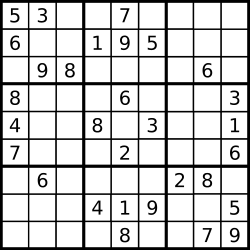
\includegraphics[width=100pt]{sudoku.png}
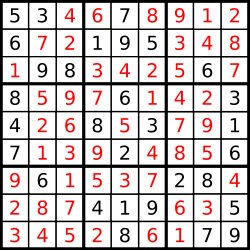
\includegraphics[width=100pt]{sudoku2.png}
\end{center}

\subsubsection{Solution}

\begin{Code}
public void solveSudoku(char[][] board) {
    if (board.length == 0) {
        return;
    }
    solve(board);
}

private boolean solve(char[][] board) {
    for (int i = 0; i < board.length; i++) {
        for (int j = 0; j < board[0].length; j++) {
            if (board[i][j] == '.') {
                for (char c = '1'; c <= '9'; c++) {
                    if (check(board, i, j, c)) {
                        board[i][j] = c;

                        if (solve(board)) {
                            return true;
                        } else {
                            board[i][j] = '.';
                        }
                    }
                }
                return false;
            }
        }
    }
    return true;
}
\end{Code}

\newpage

\begin{Code}
private boolean check(char[][] board, int row, int col, char c) {
    for (int i = 0; i < 9; i++) {
        if (board[row][i] == c) {
            return false;
        }
        if (board[i][col] == c) {
            return false;
        }

        int m = (row / 3) * 3 + i / 3;
        int n = (col / 3) * 3 + i % 3;

        if (board[m][n] == c) {
            return false;
        }
    }
    return true;
}
\end{Code}

\newpage

\section{solution.Combinations} %%%%%%%%%%%%%%%%%%%%%%

\subsubsection{Description}

Given two integers n and k, return all possible combinations of k numbers out of 1 ... n.

For example,

If n = 4 and k = 2, a solution is:
\begin{Code}
[
  [2,4],
  [3,4],
  [2,3],
  [1,2],
  [1,3],
  [1,4],
]
\end{Code}

\subsubsection{Solution}

\begin{Code}
public List<List<Integer>> combine(int n, int k) {
    List<List<Integer>> result = new ArrayList<List<Integer>>();
    List<Integer> path = new ArrayList<Integer>();
    combine(n, k, result, path, 1);
    return result;
}

private void combine(int n, int k, List<List<Integer>> result, List<Integer> path, int start) {
    if (k == 0) {
        result.add(new ArrayList<Integer>(path));
        return;
    }

    if (start > n) {
        return;
    }

    path.add(start);
    combine(n, k - 1, result, path, start + 1);
    path.remove(path.size() - 1);

    combine(n, k, result, path, start + 1);
}
\end{Code}

\newpage

\section{Restore IP Addresses} %%%%%%%%%%%%%%%%%%%%%%

\subsubsection{Description}

Given a string containing only digits, restore it by returning all possible valid IP address combinations.

For example:

Given \code{"25525511135"},

return \code{["255.255.11.135", "255.255.111.35"]}. (Order does not matter)

\subsubsection{Solution}

\begin{Code}
/**
 * 注意,0可以,但是00,01, 010这种是不允许的
 */
public List<String> restoreIpAddresses(String s) {
    List<String> list = new LinkedList<>();
    dfs(s, list, 0, 0, "");
    return list;
}

private void dfs(String s, List<String> list, int index, int count, String cur) {
    if (index >= s.length()) {
        if (count == 4) {
            list.add(cur);
        }
        return;
    }

    if (count == 4) {
        return;
    }

    int[][] RANGES = {
            {0, 0}, {0, 9}, {10, 99}, {100, 255}
    };
    for (int i = 1; i <= 3 && index + i <= s.length(); i++) {
        String t = s.substring(index, index + i);
        int n = Integer.parseInt(t);
        if (n >= RANGES[i][0] && n <= RANGES[i][1]) {
            dfs(s, list, index + i, count + 1, (cur.isEmpty() ? "" : cur + ".") + t);
        }
    }
}
\end{Code}

\newpage

\section{Word Ladder} %%%%%%%%%%%%%%%%%%%%%%

\subsubsection{Description}

Given two words (beginWord and endWord), and a dictionary's word list, find the length of shortest transformation sequence from beginWord to endWord, such that:

Only one letter can be changed at a time.

Each transformed word must exist in the word list. Note that beginWord is not a transformed word.

For example,

Given:

beginWord = \code{"hit"}

endWord = \code{"cog"}

wordList = \code{["hot","dot","dog","lot","log","cog"]}

As one shortest transformation is \code{"hit" -> "hot" -> "dot" -> "dog" -> "cog"},

return its length 5.

\textbf{Note:}

Return 0 if there is no such transformation sequence.

All words have the same length.

All words contain only lowercase alphabetic characters.

You may assume no duplicates in the word list.

You may assume beginWord and endWord are non-empty and are not the same.

\newpage

\subsubsection{Solution I}

\begin{Code}
/**
 * 要注意添加节点时要给单词从dict中删掉
 */
// 常规的BFS,耗时141ms
public int ladderLength(String beginWord, String endWord, Set<String> wordList) {
    wordList.remove(beginWord);
    wordList.add(endWord);

    Queue<String> queue = new LinkedList<>();
    Queue<String> next = new LinkedList<>();
    queue.add(beginWord);

    int ladder = 1;

    while (!queue.isEmpty()) {
        String word = queue.poll();

        StringBuilder sb = new StringBuilder(word);
        for (int i = 0; i < word.length(); i++) {
            char c = word.charAt(i);
            for (int j = 0; j < 26; j++) {
                if (j + 'a' == c) {
                    continue;
                }
                sb.setCharAt(i, (char) (j + 'a'));
                String s = sb.toString();

                if (s.equals(endWord)) {
                    return ladder + 1;
                }

                if (wordList.remove(s)) {
                    next.add(s);
                }
            }
            sb.setCharAt(i, c);
        }

        if (queue.isEmpty()) {
            queue.addAll(next);
            next.clear();
            ladder++;
        }
    }

    return 0;
}
\end{Code}

\newpage

\subsubsection{Solution II}

\begin{Code}
// 采用双端BFS,耗时28ms
public int ladderLength2(String beginWord, String endWord, Set<String> wordList) {
    Set<String> beginSet = new HashSet<>();
    beginSet.add(beginWord);

    Set<String> endSet = new HashSet<String>();
    endSet.add(endWord);

    int length = 1;

    while (!beginSet.isEmpty() && !endSet.isEmpty()) {
        if (beginSet.size() > endSet.size()) {
            Set<String> temp = beginSet;
            beginSet = endSet;
            endSet = temp;
        }

        Set<String> nextSet = new HashSet<String>();

        for (String word : beginSet) {
            char[] wordArr = word.toCharArray();

            for (int i = 0; i < wordArr.length; i++) {
                char c = wordArr[i];

                for (int j = 0; j < 26; j++) {
                    if ('a' + j == c) {
                        continue;
                    }
                    wordArr[i] = (char) ('a' + j);
                    String s = String.valueOf(wordArr);

                    if (endSet.contains(s)) {
                        return length + 1;
                    }

                    if (wordList.contains(s)) {
                        nextSet.add(s);
                        wordList.remove(s);
                    }
                }
                wordArr[i] = c;
            }
        }

        beginSet = nextSet;
        length++;
    }

    return 0;
}
\end{Code}

\newpage

\section{Word Ladder II} %%%%%%%%%%%%%%%%%%%%%%

\subsubsection{Description}
Given two words (beginWord and endWord), and a dictionary's word list, find all shortest transformation sequence(s) from beginWord to endWord, such that:

1. Only one letter can be changed at a time

2. Each transformed word must exist in the word list. Note that beginWord is not a transformed word.

For example,

Given:

beginWord = \code{"hit"}

endWord = \code{"cog"}

wordList = \code{["hot","dot","dog","lot","log","cog"]}

Return
\begin{Code}
  [
    ["hit","hot","dot","dog","cog"],
    ["hit","hot","lot","log","cog"]
  ]
\end{Code}

Note:

Return an empty list if there is no such transformation sequence.

All words have the same length.

All words contain only lowercase alphabetic characters.

You may assume no duplicates in the word list.

You may assume beginWord and endWord are non-empty and are not the same.

\subsubsection{Analysis}
这题核心就是保存前驱节点

\subsubsection{Solution}

\begin{Code}
/**
 * 保存前驱节点
 */
class WordNode {
    String word;
    WordNode prev;

    public WordNode(String word, WordNode pre) {
        this.word = word;
        this.prev = pre;
    }
}
\end{Code}

\newpage

\begin{Code}
public List<List<String>> findLadders(String beginWord, String endWord, Set<String> wordList) {
    List<List<String>> result = new ArrayList<List<String>>();
    LinkedList<WordNode> next = new LinkedList<>();
    HashSet<String> visited = new HashSet<String>();
    LinkedList<WordNode> queue = new LinkedList<WordNode>();
    queue.add(new WordNode(beginWord, null));

    wordList.remove(beginWord);
    wordList.add(endWord);

    while (!queue.isEmpty()) {
        WordNode top = queue.poll();
        String word = top.word;

        if (word.equals(endWord)) {
            ArrayList<String> t = new ArrayList<String>();
            for (WordNode p = top; p != null; p = p.prev) {
                t.add(0, p.word);
            }
            result.add(t);
            continue;
        }

        if (!result.isEmpty() && queue.isEmpty()) {
            break;
        }

        StringBuilder sb = new StringBuilder(word);
        for (int i = 0; i < word.length(); i++) {
            char c = word.charAt(i);
            for (int j = 0; j < 26; j++) {
                if ('a' + j == c) {
                    continue;
                }
                sb.setCharAt(i, (char) ('a' + j));
                String newWord = sb.toString();
                if (wordList.contains(newWord)) {
                    next.add(new WordNode(newWord, top));
                    visited.add(newWord);
                }
            }
            sb.setCharAt(i, c);
        }

        if (queue.isEmpty()) {
            queue.addAll(next);
            next.clear();
            wordList.removeAll(visited);
        }
    }

    return result;
}
\end{Code}

\newpage

\section{Palindrome Partitioning} %%%%%%%%%%%%%%%%%%%%%%

\subsubsection{Description}

Given a string s, partition s such that every substring of the partition is a palindrome.

Return all possible palindrome partitioning of s.

For example, given s = \code{"aab"},

Return
\begin{Code}
[
  ["aa","b"],
  ["a","a","b"]
]
\end{Code}

\subsubsection{Solution}

\begin{Code}
public List<List<String>> partition(String s) {
    int n = s.length();
    List<List<String>>[] f = new LinkedList[n + 1];
    f[0] = new LinkedList<List<String>>();
    f[0].add(Collections.EMPTY_LIST);

    boolean[][] flag = new boolean[n][n];
    for (int i = 0; i < n; i++) {
        f[i + 1] = new LinkedList<List<String>>();
        for (int j = 0; j <= i; j++) {
            if (s.charAt(j) == s.charAt(i) && (j > i - 2 || flag[j + 1][i - 1])) {
                flag[j][i] = true;
                for (List<String> list : f[j]) {
                    List<String> list2 = new LinkedList<String>(list);
                    list2.add(s.substring(j, i + 1));
                    f[i + 1].add(list2);
                }
            }
        }
    }

    return f[n];
}
\end{Code}

\newpage

\section{Palindrome Partitioning II} %%%%%%%%%%%%%%%%%%%%%%

\subsubsection{Description}

Given a string s, partition s such that every substring of the partition is a palindrome.

Return the minimum cuts needed for a palindrome partitioning of s.

For example, given s = \code{"aab"},

Return 1 since the palindrome partitioning \code{["aa","b"]} could be produced using 1 cut.

\subsubsection{Solution}

\begin{Code}
/**
 * 这里cuts[0]=-1是为了兼容j=i=0的情况
 */
public int minCut(String s) {
    int n = s.length();
    int[] cuts = new int[n + 1];
    cuts[0] = -1;
    boolean[][] f = new boolean[n][n];
    for (int i = 0; i < n; i++) {
        int cut = Integer.MAX_VALUE;
        for (int j = 0; j <= i; j++) {
            if (s.charAt(j) == s.charAt(i) && (j > i - 2 || f[j + 1][i - 1])) {
                f[j][i] = true;
                cut = Math.min(cut, cuts[j] + 1);
            }
        }
        cuts[i + 1] = cut;
    }
    return cuts[n];
}
\end{Code}

\newpage

\section{Palindrome Permutation} %%%%%%%%%%%%%%%%%%%%%%

\subsubsection{Description}

Given a string, determine if a permutation of the string could form a palindrome.

For example, \code{"code" -> False, "aab" -> True, "carerac" -> True}.

\subsubsection{Solution}

\begin{Code}
public boolean canPermutePalindrome(String s) {
    int len = s.length();
    int[] count = new int[256];
    for (char c : s.toCharArray()) {
        count[c]++;
    }
    int num = 0;
    for (int i = 0; i < count.length; i++) {
        num += (count[i] >> 1) << 1;
    }
    if (num < len) {
        num++;
    }
    return num == len;
}
\end{Code}

\newpage

\section{Palindrome Permutation II} %%%%%%%%%%%%%%%%%%%%%%

\subsubsection{Description}
Given a string s, return all the palindromic permutations (without duplicates) of it. Return an empty list if no palindromic permutation could be form.

For example:

Given s = \code{"aabb"}, return \code{["abba", "baab"]}.

Given s = \code{"abc"}, return [].

\subsubsection{Solution}
\begin{Code}
public static List<String> generatePalindromes(String s) {
    int[] counts = new int[256];
    for (char c : s.toCharArray()) {
        counts[c]++;
    }

    List<String> list = new LinkedList<>();
    StringBuilder sb = new StringBuilder();

    char single = 0;
    for (int i = 0; i < counts.length; i++) {
        if (counts[i] % 2 != 0) {
            if (single != 0) {
                return list;
            }
            single = (char) i;
            counts[i] = ((counts[i] >> 1) << 1);
        }
        for (int j = 0; j < counts[i]; j += 2) {
            sb.append((char)i);
        }
    }

    helper(sb, "" + (single != 0 ? single : ""), list);
    return list;
}

private static void helper(StringBuilder sb, String cur, List<String> list) {
    if (sb.length() == 0) {
        list.add(cur);
        return;
    }
    for (int i = 0; i < sb.length(); i++) {
        if (i > 0 && sb.charAt(i) == sb.charAt(i - 1)) {
            continue;
        }
        char c = sb.charAt(i);
        sb.deleteCharAt(i);
        helper(sb, c + cur + c, list);
        sb.insert(i, c);
    }
}
\end{Code}

\newpage

\section{Generalized Abbreviation} %%%%%%%%%%%%%%%%%%%%%%

\subsubsection{Description}
Write a function to generate the generalized abbreviations of a word.

\textbf{Example:}

Given word = "word", return the following list (order does not matter):

\code{["word", "1ord", "w1rd", "wo1d", "wor1", "2rd", "w2d", "wo2", "1o1d", "1or1", "w1r1", "1o2", "2r1", "3d", "w3", "4"]}

\subsubsection{Solution}

\begin{Code}
public List<String> generateAbbreviations(String word) {
    List<String> list = new LinkedList<>();
    helper(word, 0, list, "", 0);
    return list;
}

private void helper(String word, int idx, List<String> list, String cur, int count) {
    if (idx == word.length()) {
        if (count > 0) {
            cur += count;
        }
        list.add(cur);
        return;
    }

    helper(word, idx + 1, list, cur, count + 1);
    helper(word, idx + 1, list, cur + (count > 0 ? count : "") + word.charAt(idx), 0);
}
\end{Code}

\newpage

\section{Binary Watch} %%%%%%%%%%%%%%%%%%%%%%

\subsubsection{Description}

A binary watch has 4 LEDs on the top which represent the hours (0-11), and the 6 LEDs on the bottom represent the minutes (0-59).

Each LED represents a zero or one, with the least significant bit on the right.

\begin{center}
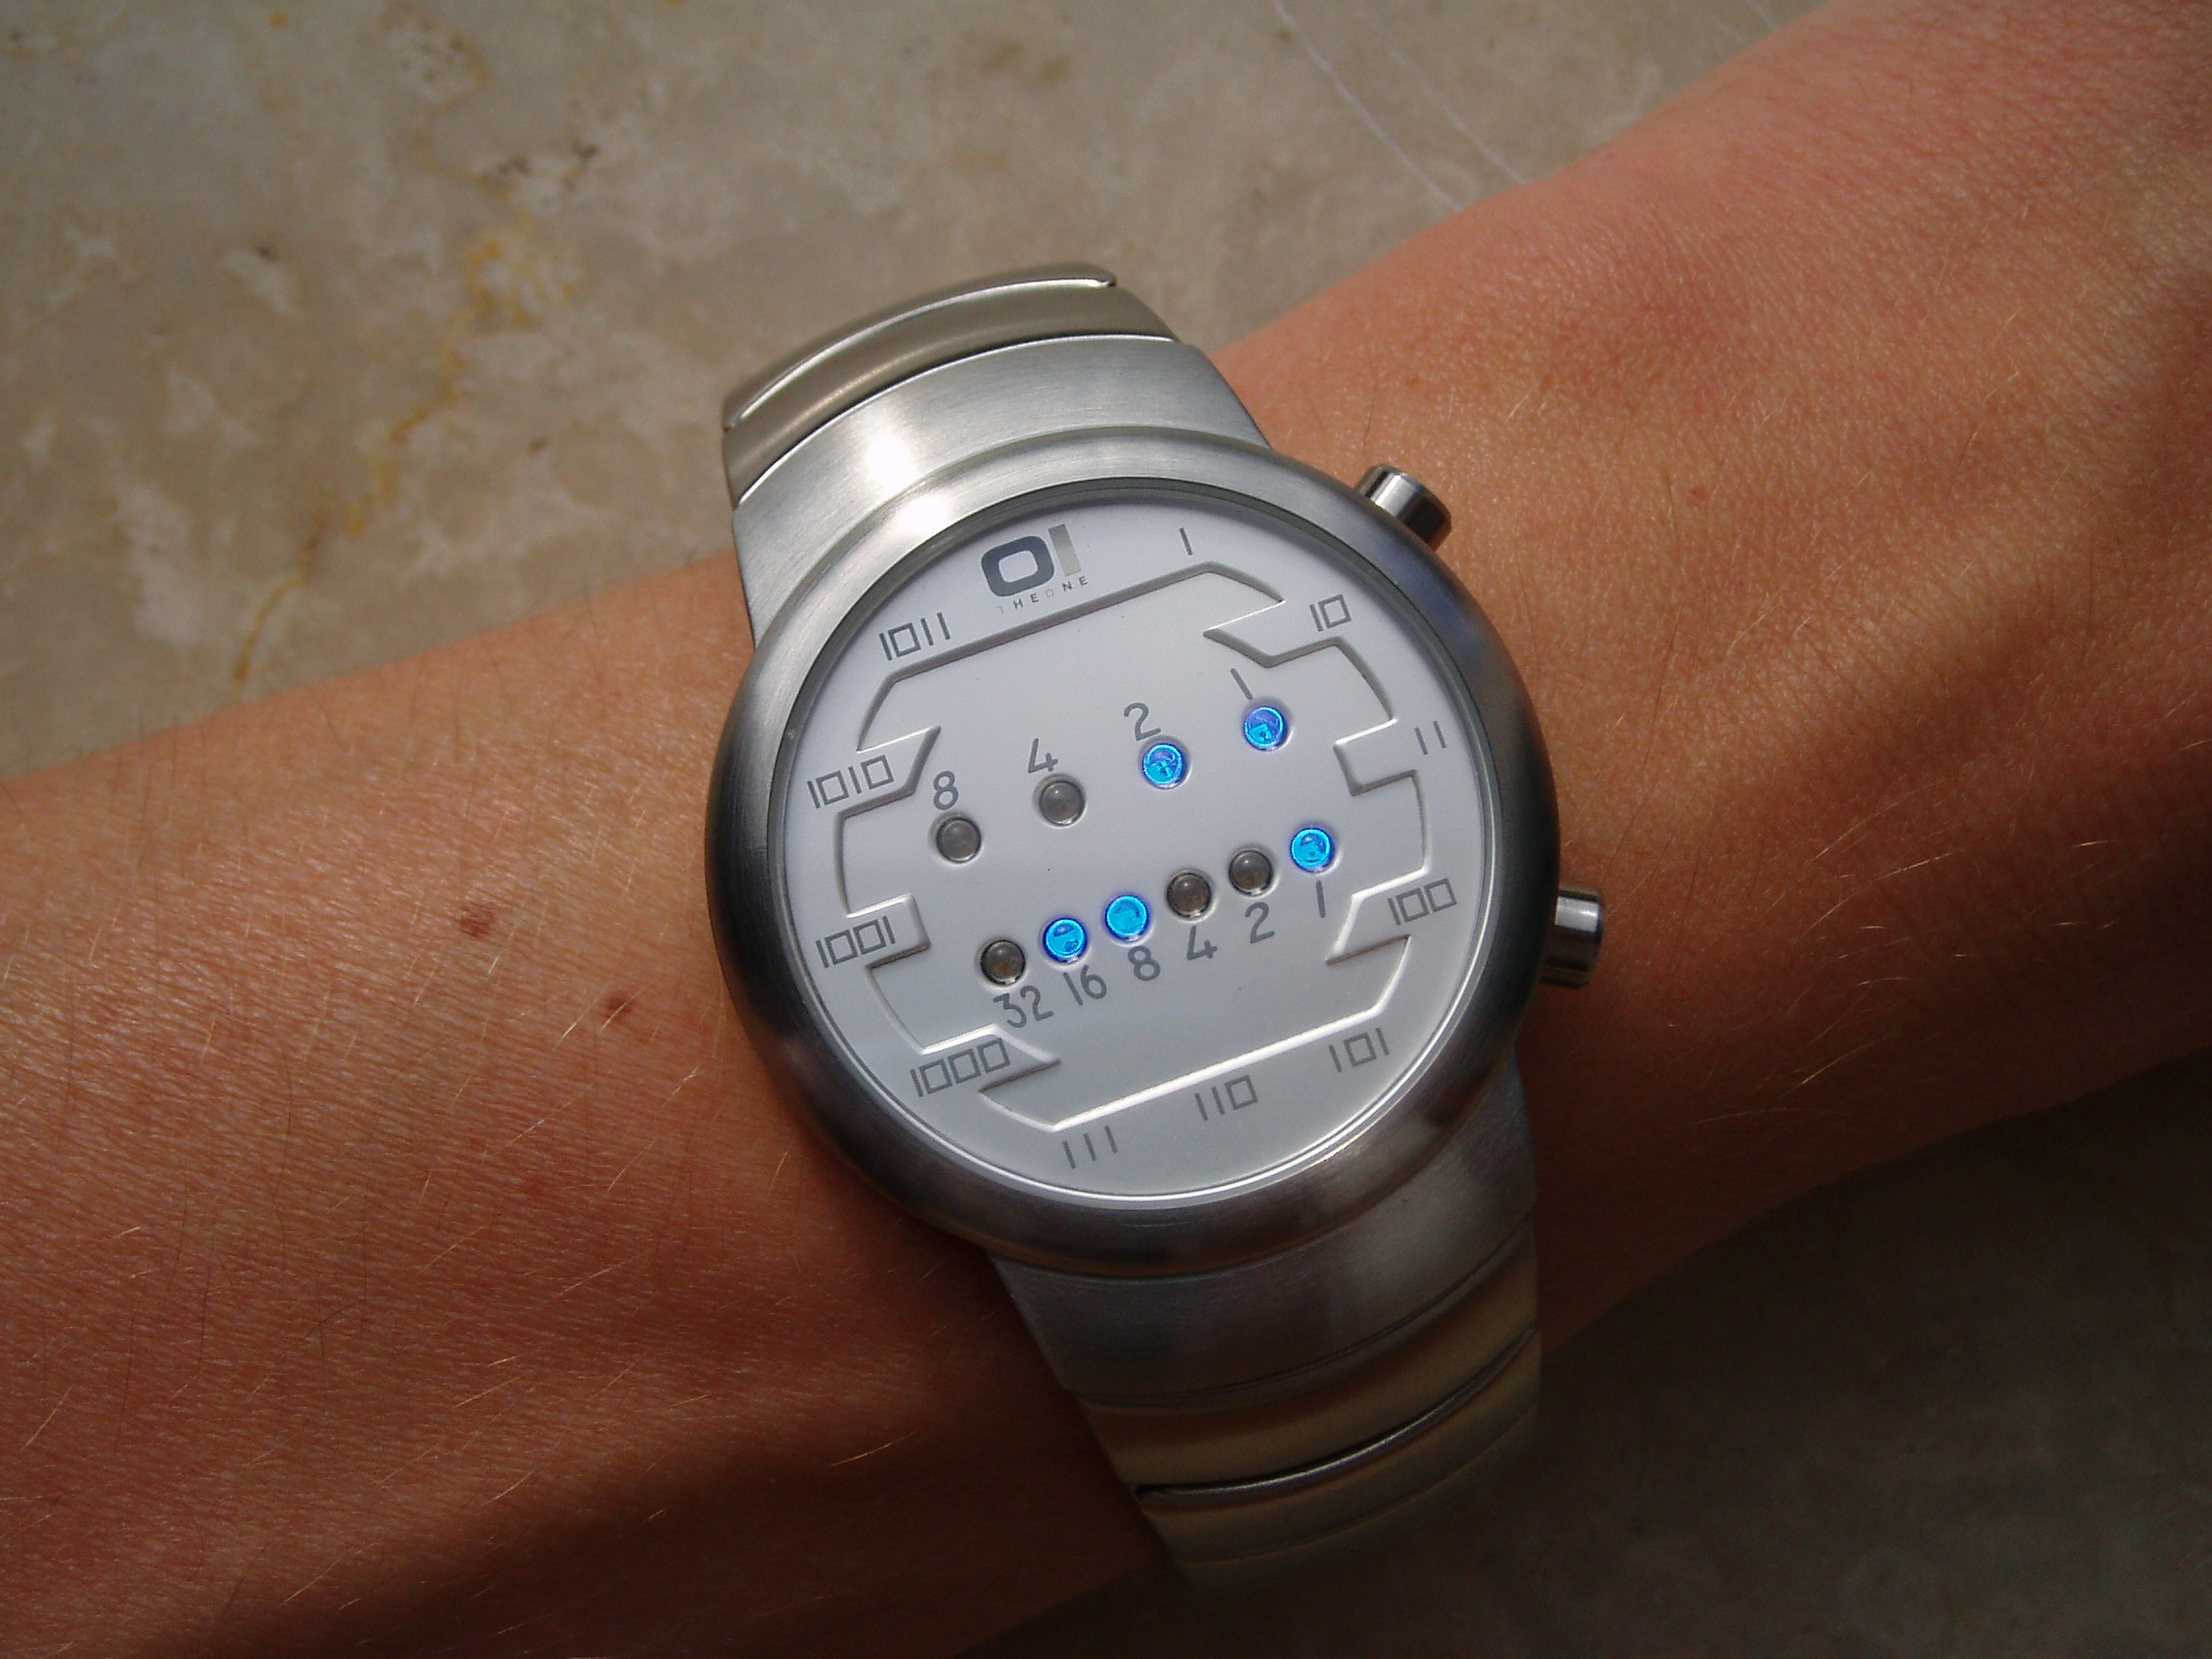
\includegraphics[width=150pt]{watch.jpg}\\
\end{center}

For example, the above binary watch reads \code{"3:25"}.

Given a non-negative integer n which represents the number of LEDs that are currently on, return all possible times the watch could represent.

\textbf{Example:}

\textbf{Input:} n = 1

\textbf{Return:} \code{["1:00", "2:00", "4:00", "8:00", "0:01", "0:02", "0:04", "0:08", "0:16", "0:32"]}

\textbf{Note:}

The order of output does not matter.

The hour must not contain a leading zero, for example \code{"01:00"} is not valid, it should be \code{"1:00"}.

The minute must be consist of two digits and may contain a leading zero, for example \code{"10:2"} is not valid, it should be \code{"10:02"}.

\subsubsection{Solution}
\begin{Code}
public List<String> readBinaryWatch(int num) {
    int[] f = new int[] {
            1, 2, 4, 8, 1, 2, 4, 8, 16, 32
    };

    List<String> list = new ArrayList<String>();
    readBinaryWatch(num, f, 0, 0, 0, list);

    return list;
}
\end{Code}

\newpage

\begin{Code}
public void readBinaryWatch(int num, int[] f, int index, int hour, int minute, List<String> list) {
    if (num == 0 && hour < 12 && minute < 60) {
        list.add(String.format("%d:%02d", hour, minute));
        return;
    }

    if (index >= f.length) {
        return;
    }

    int nextHour = index <= 3 ? hour + f[index] : hour;
    int nextMinute = index > 3 ? minute + f[index] : minute;
    readBinaryWatch(num - 1, f, index + 1, nextHour, nextMinute, list);
    readBinaryWatch(num, f, index + 1, hour, minute, list);
}
\end{Code}

\newpage

\section{Add and Search Word} %%%%%%%%%%%%%%%%%%%%%%

\subsubsection{Description}

Design a data structure that supports the following two operations:
\begin{Code}
void addWord(word)
bool search(word)
\end{Code}
search(word) can search a literal word or a regular expression string containing only letters a-z or .. A . means it can represent any one letter.

For example:
\begin{Code}
addWord("bad")
addWord("dad")
addWord("mad")
search("pad") -> false
search("bad") -> true
search(".ad") -> true
search("b..") -> true
\end{Code}
\textbf{Note:}

You may assume that all words are consist of lowercase letters a-z.

\subsubsection{Solution}

\begin{Code}
TriNode root;

class TriNode {
    TriNode[] nodes = new TriNode[26];
    String word;
}

public AddAndSearchWord() {
    root = new TriNode();
}

public void addWord(String word) {
    TriNode node = root;
    for (char c : word.toCharArray()) {
        if (node.nodes[c - 'a'] == null) {
            node.nodes[c - 'a'] = new TriNode();
        }
        node = node.nodes[c - 'a'];
    }
    node.word = word;
}

public boolean search(String word) {
    return search(root, word);
}

\end{Code}

\newpage
\begin{Code}
private boolean search(TriNode node, String word) {
    if (node == null) {
        return false;
    }

    for (int i = 0; i < word.length(); i++) {
        char c = word.charAt(i);

        if (c != '.') {
            if (node.nodes[c - 'a'] == null) {
                return false;
            }
            node = node.nodes[c - 'a'];
        } else {
            String s = word.substring(i + 1);
            for (char cc = 'a'; cc <= 'z'; cc++) {
                if (search(node.nodes[cc - 'a'], s)) {
                    return true;
                }
            }
            return false;
        }
    }

    return node.word != null;
}
\end{Code}

\newpage

\section{Factor solution.Combinations} %%%%%%%%%%%%%%%%%%%%%%
\subsubsection{Descriptor}
Numbers can be regarded as product of its factors. For example,
\begin{Code}
8 = 2 x 2 x 2;
  = 2 x 4.
\end{Code}
Write a function that takes an integer n and return all possible combinations of its factors.

\textbf{Note:}

You may assume that n is always positive.

Factors should be greater than 1 and less than n.

\textbf{Examples:}

\textbf{input:} 1

\textbf{output:} \code{[]}

\textbf{input:} 37

\textbf{output:} \code{[]}

\textbf{input:} 12

\textbf{output:}

\begin{Code}
[
  [2, 6],
  [2, 2, 3],
  [3, 4]
]
\end{Code}

\textbf{input:} 32

\textbf{output:}

\begin{Code}
[
  [2, 16],
  [2, 2, 8],
  [2, 2, 2, 4],
  [2, 2, 2, 2, 2],
  [2, 4, 4],
  [4, 8]
]
\end{Code}

\newpage

\subsubsection{Solution}
\begin{Code}
public List<List<Integer>> getFactors(int n) {
    List<List<Integer>> result = new LinkedList<>();
    dfs(n, 2, result, new LinkedList<>());
    return result;
}

private void dfs(int n, int cur, List<List<Integer>> result, List<Integer> list) {
    if (n <= 1) {
        if (list.size() > 1) {
            result.add(new LinkedList<>(list));
        }
        return;
    }

    for (int i = cur; i <= n; i++) {
        if (n % i == 0) {
            list.add(i);
            dfs(n / i, i, result, list);
            list.remove(list.size() - 1);
        }
    }
}
\end{Code}

\newpage

\section{Valid Word Square} %%%%%%%%%%%%%%%%%%%%%%

\subsubsection{Description}
Given a sequence of words, check whether it forms a valid word square.

A sequence of words forms a valid word square if the kth row and column read the exact same string, where 0 <= k < max(numRows, numColumns).

\textbf{Note:}

1. The number of words given is at least 1 and does not exceed 500.

2. Word length will be at least 1 and does not exceed 500.

3. Each word contains only lowercase English alphabet a-z.

\textbf{Example:}

\textbf{Input:}

\begin{Code}
[
  "abcd",
  "bnrt",
  "crmy",
  "dtye"
]
\end{Code}

\textbf{Output:}

true

\textbf{Explanation:}

The first row and first column both read "abcd".

The second row and second column both read "bnrt".

The third row and third column both read "crmy".

The fourth row and fourth column both read "dtye".

Therefore, it is a valid word square.

\subsubsection{Solution}
\begin{Code}
public boolean validWordSquare(List<String> words) {
    for (int i = 0; i < words.size(); i++) {
        String word = words.get(i);
        if (word.length() > words.size()) {
            return false;
        }
        for (int j = 0; j < word.length(); j++) {
            String s = words.get(j);
            if (i >= s.length() || word.charAt(j) != s.charAt(i)) {
                return false;
            }
        }
    }
    return true;
}
\end{Code}

\newpage

\section{Word Squares} %%%%%%%%%%%%%%%%%%%%%%
\subsubsection{Description}
Given a set of words (without duplicates), find all word squares you can build from them.

A sequence of words forms a valid word square if the kth row and column read the exact same string, where 0 <= k < max(numRows, numColumns).

For example, the word sequence \code{["ball","area","lead","lady"]} forms a word square because each word reads the same both horizontally and vertically.

\begin{Code}
b a l l
a r e a
l e a d
l a d y
\end{Code}

\textbf{Note:}

1. There are at least 1 and at most 1000 words.

2. All words will have the exact same length.

3. Word length is at least 1 and at most 5.

4. Each word contains only lowercase English alphabet a-z.


\textbf{Example:}

\textbf{Input:}

\code{["area","lead","wall","lady","ball"]}

\textbf{Output:}
\begin{Code}
[
  [ "wall",
    "area",
    "lead",
    "lady"
  ],
  [ "ball",
    "area",
    "lead",
    "lady"
  ]
]
\end{Code}
\textbf{Explanation:}

The output consists of two word squares. The order of output does not matter (just the order of words in each word square matters).
\newpage

\subsubsection{Solution}
\begin{Code}
public List<List<String>> wordSquares(String[] words) {
    List<List<String>> ret = new ArrayList<List<String>>();
    if (words.length == 0 || words[0].length() == 0) {
        return ret;
    }
    Map<String, Set<String>> map = new HashMap<>();
    int squareLen = words[0].length();
    for (int i = 0; i < words.length; i++) {
        /**
         * 注意这里空字符也算前缀,所以j从-1开始
         */
        for (int j = -1; j < words[0].length(); j++) {
            String prefix = words[i].substring(0, j + 1);
            Set<String> set = map.get(prefix);
            if (set == null) {
                set = new HashSet<String>();
                map.put(prefix, set);
            }
            set.add(words[i]);
        }
    }
    helper(ret, new ArrayList<String>(), squareLen, map);
    return ret;
}

public void helper(List<List<String>> ret, List<String> cur, int total, Map<String, Set<String>> map) {
    if (cur.size() == total) {
        ret.add(new ArrayList<String>(cur));
        return;
    }
    // build search string
    StringBuilder sb = new StringBuilder();
    for (int i = 0; i < cur.size(); i++) {
        /**
         * 下一个单词的prefix必然是当前这些单词的第cur.size列
         */
        sb.append(cur.get(i).charAt(cur.size()));
    }
    // bachtracking
    Set<String> cand = map.get(sb.toString());
    if (cand == null) {
        return;
    }
    for (String str : cand) {
        cur.add(str);
        helper(ret, cur, total, map);
        cur.remove(cur.size() - 1);
    }
}
\end{Code}

\newpage

\section{Beautiful Arrangement} %%%%%%%%%%%%%%%%%%%%%%
\subsubsection{Description}

Suppose you have N integers from 1 to N. We define a beautiful arrangement as an array that is constructed by these N numbers successfully if one of the following is true for the ith position (1 <= i <= N) in this array:

1. The number at the ith position is divisible by i.

2. i is divisible by the number at the ith position.

Now given N, how many beautiful arrangements can you construct?

\textbf{Example:}

\textbf{Input: 2}

\textbf{Output: 2}

\textbf{Explanation:}

The first beautiful arrangement is [1, 2]:

Number at the 1st position (i=1) is 1, and 1 is divisible by i (i=1).

Number at the 2nd position (i=2) is 2, and 2 is divisible by i (i=2).

The second beautiful arrangement is [2, 1]:

Number at the 1st position (i=1) is 2, and 2 is divisible by i (i=1).

Number at the 2nd position (i=2) is 1, and i (i=2) is divisible by 1.

\textbf{Note:}

N is a positive integer and will not exceed 15.

\subsubsection{Solution}
\begin{Code}
public int countArrangement(int N) {
    int[] count = new int[1];
    helper(N, 1, new boolean[N + 1], count);
    return count[0];
}

private void helper(int N, int k, boolean[] visited, int[] count) {
    if (k > N) {
        count[0]++;
        return;
    }

    for (int i = 1; i <= N; i++) {
        if (!visited[i] && (i % k == 0 || k % i == 0)) {
            visited[i] = true;
            helper(N, k + 1, visited, count);
            visited[i] = false;
        }
    }
}
\end{Code}

\newpage

\section{Flip Game} %%%%%%%%%%%%%%%%%%%%%%
\subsubsection{Description}

You are playing the following Flip Game with your friend: Given a string that contains only these two characters: + and -, you and your friend take turns to flip two consecutive \code{"++"} into \code{"--"}. The game ends when a person can no longer make a move and therefore the other person will be the winner.

Write a function to compute all possible states of the string after one valid move.

For example, given s = \code{"++++"}, after one move, it may become one of the following states:

\begin{Code}
[
  "--++",
  "+--+",
  "++--"
]
\end{Code}

If there is no valid move, return an empty list [].

\subsubsection{Solution}

\begin{Code}
public List<String> generatePossibleNextMoves(String s) {
    List<String> result = new LinkedList<>();
    for (int i = 0; i < s.length(); ) {
        int index = s.indexOf("++", i);
        if (index >= i) {
            result.add(s.substring(0, index) + "--" + s.substring(index + 2));
            i = index + 1;
        } else {
            break;
        }
    }
    return result;
}
\end{Code}

\newpage

\section{Flip Game II} %%%%%%%%%%%%%%%%%%%%%%
\subsubsection{Description}

You are playing the following Flip Game with your friend: Given a string that contains only these two characters: + and -, you and your friend take turns to flip two consecutive \code{"++"} into \code{"--"}. The game ends when a person can no longer make a move and therefore the other person will be the winner.

Write a function to determine if the starting player can guarantee a win.

For example, given s = \code{"++++"}, return true. The starting player can guarantee a win by flipping the middle \code{"++"} to become \code{"+--+"}.

\textbf{Follow up:}

Derive your algorithm's runtime complexity.

\subsubsection{Solution}

\begin{Code}
public boolean canWin(String s) {
    for (int i = 0; i < s.length(); ) {
        int index = s.indexOf("++", i);
        if (index >= i) {
            String t = s.substring(0, index) + "--" + s.substring(index + 2);
            if (!canWin(t)) {
                return true;
            }
            i = index + 1;
        } else {
            break;
        }
    }
    return false;
}
\end{Code}

\newpage

\section{Android Unlock Patterns} %%%%%%%%%%%%%%%%%%%%%%
\subsubsection{Description}

Given an Android 3x3 key lock screen and two integers m and n, where 1 ≤ m ≤ n ≤ 9, count the total number of unlock patterns of the Android lock screen, which consist of minimum of m keys and maximum n keys.

\textbf{Rules for a valid pattern:}

1. Each pattern must connect at least m keys and at most n keys.

2. All the keys must be distinct.

3. If the line connecting two consecutive keys in the pattern passes through any other keys, the other keys must have previously selected in the pattern. No jumps through non selected key is allowed.

4. The order of keys used matters.

\begin{center}
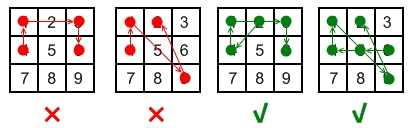
\includegraphics[width=200pt]{unlock.png}\\
\end{center}

\textbf{Explanation:}
\begin{Code}
| 1 | 2 | 3 |
| 4 | 5 | 6 |
| 7 | 8 | 9 |
\end{Code}

\textbf{Invalid move:} \code{4 - 1 - 3 - 6}

Line \code{1 - 3} passes through key 2 which had not been selected in the pattern.

\textbf{Invalid move:} \code{4 - 1 - 9 - 2}

Line \code{1 - 9} passes through key 5 which had not been selected in the pattern.

\textbf{Valid move:} \code{2 - 4 - 1 - 3 - 6}

Line \code{1 - 3} is valid because it passes through key 2, which had been selected in the pattern

\textbf{Valid move:} \code{6 - 5 - 4 - 1 - 9 - 2}

Line \code{1 - 9} is valid because it passes through key 5, which had been selected in the pattern.

\textbf{Example:}

Given m = 1, n = 1, return 9.

\newpage

\subsubsection{Solution}
\begin{Code}
int DFS(boolean vis[], int[][] skip, int cur, int remain) {
    if(remain < 0) return 0;
    if(remain == 0) return 1;
    vis[cur] = true;
    int rst = 0;
    for(int i = 1; i <= 9; ++i) {
        // If vis[i] is not visited and (two numbers are adjacent or skip number is already visited)
        if(!vis[i] && (skip[cur][i] == 0 || (vis[skip[cur][i]]))) {
            rst += DFS(vis, skip, i, remain - 1);
        }
    }
    vis[cur] = false;
    return rst;
}

public int numberOfPatterns(int m, int n) {
    // Skip array represents number to skip between two pairs
    int skip[][] = new int[10][10];
    skip[1][3] = skip[3][1] = 2;
    skip[1][7] = skip[7][1] = 4;
    skip[3][9] = skip[9][3] = 6;
    skip[7][9] = skip[9][7] = 8;
    skip[1][9] = skip[9][1] = skip[2][8] = skip[8][2] = skip[3][7] = skip[7][3] = skip[4][6] = skip[6][4] = 5;
    boolean vis[] = new boolean[10];
    int rst = 0;
    // DFS search each length from m to n
    for(int i = m; i <= n; ++i) {
        rst += DFS(vis, skip, 1, i - 1) * 4;    // 1, 3, 7, 9 are symmetric
        rst += DFS(vis, skip, 2, i - 1) * 4;    // 2, 4, 6, 8 are symmetric
        rst += DFS(vis, skip, 5, i - 1);        // 5
    }
    return rst;
}
\end{Code}
\newpage